\clearpage
\section{兔子远景的网格细节}

把视口中的兔子缩小到 38 像素高，耳尖可能只占一两个像素。让显卡继续画原模型的 16\,301 个三角形，仍旧只能写进这些像素。Stanford 的原始扫描包恰好提供了同一只兔子的几份简化网格，坐标与朝向保持一致。项目选用其中三档，分别有 16\,301、3\,851 和 948 个三角形。模型从近景切换到远景时，场景中的实体、位置和覆盖材质保持一致。\href{https://graphics.stanford.edu/data/3Dscanrep/}{Stanford 模型来源}

\begin{center}
\panelimage{.43\linewidth}{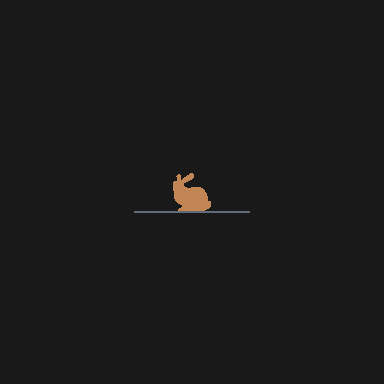
\includegraphics[width=.78\linewidth,trim=164bp 164bp 164bp 164bp,clip]{mesh-lod/Vulkan-full.png}}{LOD 0，16\,301 个三角形}
\hfill
\panelimage{.43\linewidth}{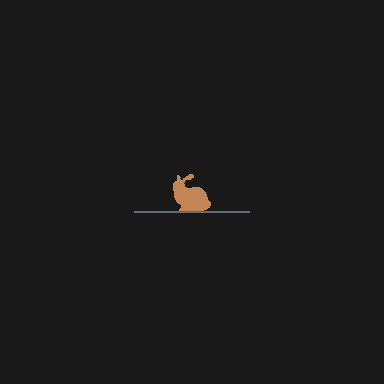
\includegraphics[width=.78\linewidth,trim=164bp 164bp 164bp 164bp,clip]{mesh-lod/Vulkan-auto.png}}{LOD 2，948 个三角形}
\end{center}
同机位的 Vulkan 基础材质实拍。原图 $384\times384$，取正中 $56\times56$ 像素放大，以便看清轮廓。耳朵和前爪仍可辨认。原网格覆盖 914 个兔子像素，简化后是 877 个；两张轮廓有 47 个像素不同，交集占并集的 94.89\%。这是此机位的取舍，模型有细长触角或镂空时，要另外检查侧面轮廓。

在层级里选中兔子，展开「属性 → 模型绘制 → 网格细节 LOD」。LOD 0 是原文件；按「添加简化模型」选择与它对齐的网格，再调「视口高度」。若使用实体的覆盖材质，各档的子网格顺序也要一致。阈值保存在场景里。示例的头两条是 25\% 与 12\%，新手可以把第一条理解为“兔子大约还占画面四分之一时换一次”。视口高 384 像素时，第一档在拉远到 $384\times0.25\times0.9=86.4$ 像素以下切换，拉近到 $384\times0.25\times1.1=105.6$ 像素以上切回。在两条线之间保留原档，轻轻来回拖相机时，耳朵就不会反复变形。

同样远的一个人和一栋楼，在屏幕上会占不同的高度。用这个比例设阈值，两件东西就能各按自己的轮廓选网格。Unity 的 LOD Group 也用对象相对于画面的高度；它可以在两档之间同时画两个模型并淡化过渡。Redflag 这里只画选中的一档，轮廓的突然变化仍要靠实际画面检查。\href{https://docs.unity3d.com/6000.0/Documentation/Manual/class-LODGroup.html}{Unity 6.0，LOD Group}

\begin{center}
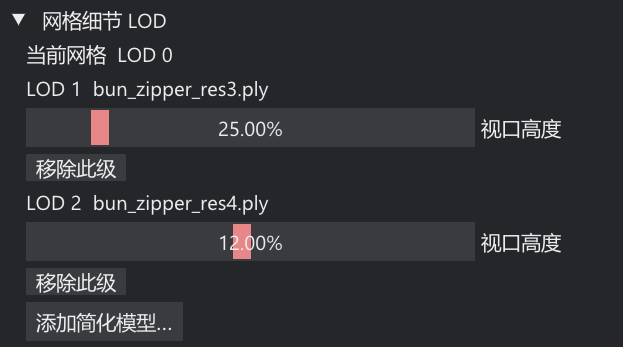
\includegraphics[width=.49\linewidth]{mesh-lod/inspector.png}\par
{\small\sffamily\color{Muted}正式编辑器的属性面板。当前用原网格，下面两行是简化模型与切换高度。}
\end{center}

\clearpage
\subsection{选定网格后的几次绘制}

导入时，\texttt{Model} 合并各部件的包围盒。绘制前，\texttt{SceneRenderer} 把原模型包围盒的八个角投影到屏幕，取最上和最下两点的高度差，得到与视口的比例。即使上一帧画了简化兔子，下一次仍用同一个原包围盒量尺寸。TAA 挪动采样位置时，选档沿用未偏移的相机。\href{run:../../Redflag/src/Redflag/Renderer/Model.cpp}{包围盒投影}\quad\href{run:../../Redflag/src/Redflag/Renderer/SceneRenderer.cpp}{场景选档和绘制}

OpenGL 场景在收集几何时选一次网格。实际截帧中，阴影、反射阴影图、深度预写和主绘制四次画兔子，远景每次都读 2\,844 个索引，保持原模型时每次读 48\,903 个。Vulkan 中，相机看到的表面、透明绘制和拾取也用同一选档。二次光线的碰撞树仍用原模型。拉远相机不会因此移动阴影遮挡物或令烘焙探针失效，但较粗的轮廓可能与精细模型投下的阴影有细微差别。

{\smalltable\noindent\begin{tabularx}{\linewidth}{@{}Xrrrr@{}}\toprule
基础材质，两次绘制（兔子与地面） & \multicolumn{2}{c}{CPU 记录两物体（微秒）}&\multicolumn{2}{c}{GPU 画兔子（微秒）}\\
\cmidrule(lr){2-3}\cmidrule(l){4-5}
后端 & 原网格 & LOD 2 & 原网格 & LOD 2\\\midrule
OpenGL & 64.40 & 52.60 & 2.400 & 0.224\\
Vulkan & 46.00 & 47.35 & 2.272 & 0.512\\\bottomrule
\end{tabularx}\par}

RTX 5070 Ti Laptop GPU、Debug x64。CPU 单独运行，每组预热四帧再记录 32 帧，表中取中位数。计时从提交场景几何开始，到记录两次绘制完成结束。每次测试都读取躯干中央的实体编号；读回在计时区间之外。GPU 时间取 RenderDoc 1.47 对同一绘制事件的九次回放中位数。三角形减少了 94.18\%，绘制调用仍是两次；Vulkan 这组 CPU 记录多用 1.35 微秒。这样的局部测量无法推算整帧能提升多少。

\noindent{\small 仓库根目录，Windows 命令。替换最后一个词为 \texttt{full}，即可用原网格作对照。}
\begin{lstlisting}
python tests/fetch_stanford.py
tests\run_mesh_lod.cmd Vulkan auto
tests\run_mesh_lod.cmd OpenGL auto
tests\run_mesh_lod.cmd OpenGLScene auto
\end{lstlisting}
各档索引数、事件编号、帧校验值和时间样本在 \path{output/profiling/mesh-lod/results.json} 与同目录的 CSV。下次可在同一位置放置多只兔子，检验几何负载增大时的整帧时间；对运动中的耳朵还可以逐帧比较档位切换前后的轮廓。
